\documentclass[border=5pt]{standalone}
\usepackage{tikz}
\usepackage{xcolor}

\begin{document}
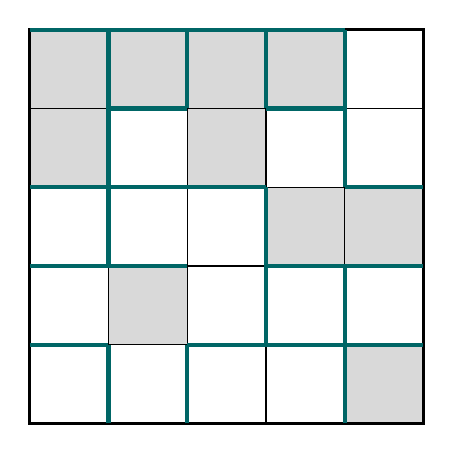
\begin{tikzpicture}

% 定义样式
\tikzset{
  cell/.style={
    rectangle,
    minimum size=1cm,
    draw=none,
    fill=#1
  },
  emphasis/.style={
    line width=1.5pt,
    teal!80!black
  }
}

% 绘制所有白色背景单元格
\foreach \i in {1,...,5} {
  \foreach \j in {1,...,5} {
    \node[cell=white] at (\i-0.5,6-\j-0.5) {};
  }
}

% 绘制灰色单元格
\node[cell=gray!30] at (0.5,4.5) {};
\node[cell=gray!30] at (1.5,4.5) {};
\node[cell=gray!30] at (2.5,4.5) {};
\node[cell=gray!30] at (3.5,4.5) {};
\node[cell=gray!30] at (0.5,3.5) {};
\node[cell=gray!30] at (2.5,3.5) {};
\node[cell=gray!30] at (3.5,2.5) {};
\node[cell=gray!30] at (4.5,2.5) {};
\node[cell=gray!30] at (1.5,1.5) {};
\node[cell=gray!30] at (4.5,0.5) {};

% 绘制常规网格线
\draw[step=1cm, black, thin] (0,0) grid (5,5);

% 绘制外边框
\draw[black, line width=1pt] (0,0) rectangle (5,5);

% 绘制强调边框
% 水平强调线
\draw[emphasis] (0,1) -- (1,1);
\draw[emphasis] (2,1) -- (5,1);
\draw[emphasis] (0,2) -- (2,2);
\draw[emphasis] (3,2) -- (5,2);
\draw[emphasis] (0,3) -- (3,3);
\draw[emphasis] (4,3) -- (5,3);
\draw[emphasis] (1,4) -- (2,4);
\draw[emphasis] (3,4) -- (4,4);
\draw[emphasis] (0,5) -- (4,5);

% 垂直强调线
\draw[emphasis] (1,0) -- (1,1);
\draw[emphasis] (1,2) -- (1,5);
\draw[emphasis] (2,0) -- (2,1);
\draw[emphasis] (2,4) -- (2,5);
\draw[emphasis] (3,1) -- (3,3);
\draw[emphasis] (3,4) -- (3,5);
\draw[emphasis] (4,0) -- (4,2);
\draw[emphasis] (4,3) -- (4,5);

\end{tikzpicture}
\end{document}